% SIAM Supplemental File Template
\documentclass[review,supplement,onefignum,onetabnum]{siamart190516}


% SIAM Shared Information Template
% This is information that is shared between the main document and any
% supplement. If no supplement is required, then this information can
% be included directly in the main document.


% Packages and macros go here
\ifpdf
  \DeclareGraphicsExtensions{.eps,.pdf,.png,.jpg}
\else
  \DeclareGraphicsExtensions{.eps}
\fi

% Add a serial/Oxford comma by default.
\newcommand{\creflastconjunction}{, and~}
\newcommand{\IP}{IP$_3$}
\newcommand{\Ca}{$\textrm{Ca}^{2+}$~}
\newcommand{\R}{\mathbb{R}}
\newcommand{\cc}{$c_c$}
\newcommand{\ce}{$c_e$}
\newcommand{\co}{$c_o$}
\newcommand{\btot}{$b^{tot}$}
\newcommand{\betot}{$b_e^{tot}$}
\newcommand{\Dc}{$D_c$}
\newcommand{\Db}{$D_b$}
\newcommand{\Dce}{$D_{ce}$}
\newcommand{\Dbe}{$D_{be}$}
\newcommand{\ER}{Endoplasmic Reticulum}

% Used for creating new theorem and remark environments
\newsiamremark{remark}{Remark}
\newsiamremark{hypothesis}{Hypothesis}
\crefname{hypothesis}{Hypothesis}{Hypotheses}
\newsiamthm{claim}{Claim}

% Sets running headers as well as PDF title and authors
\headers{A computational study of Alzheimer's disease}{P. Borole, J. M. Rosado, M. Neal, and G. Queisser}

% Title. If the supplement option is on, then "Supplementary Material"
% is automatically inserted before the title.
\title{Neuronal Resilience and Calcium Signaling Pathways in the Context of Synapse Loss and Calcium Leaks: A computational modelling study and Implications for Alzheimer's Disease\thanks{Submitted to the editors \today}}
%\funding{This work was funded by the Fog Research Institute under contract no.~FRI-454.}}}

% Authors: full names plus addresses.
\author{
Piyush Borole\thanks{University of Edinburgh, Edinburgh, Scotland, United Kingdom}
\and James M. Rosado\thanks{Department of Mathematics, Temple University, Philadelphia, Pennsylvania, U.S.A.}
\and MeiRose Neal\footnotemark[3]
 \and Gillian Queisser\footnotemark[3] 
}
\usepackage{amsopn}
\DeclareMathOperator{\diag}{diag}

%%% Local Variables: 
%%% mode:latex
%%% TeX-master: "ex_article"
%%% End: 

\usepackage{mathtools}
%%%%%
\usepackage{xr}
\makeatletter

\newcommand*{\addFileDependency}[1]{% argument=file name and extension
\typeout{(#1)}% latexmk will find this if $recorder=0
% however, in that case, it will ignore #1 if it is a .aux or 
% .pdf file etc and it exists! If it doesn't exist, it will appear 
% in the list of dependents regardless)
%
% Write the following if you want it to appear in \listfiles 
% --- although not really necessary and latexmk doesn't use this
%
%\@addtofilelist{#1}
%
% latexmk will find this message if #1 doesn't exist (yet)
\IfFileExists{#1}{}{\typeout{No file #1.}}
}\makeatother

\newcommand*{\myexternaldocument}[1]{%
\externaldocument[nocite]{#1}%
\addFileDependency{#1.tex}%
\addFileDependency{#1.aux}%
}
%------------End of helper code--------------
% put all the external documents here!
\myexternaldocument{ex_article}
%\externaldocument[nocite]{ex_article}
% Optional PDF information
\ifpdf
\hypersetup{
  pdftitle={A computational study of Alzheimer's disease using a coupled electro-calcium model},
  pdfauthor={P. Borole, J. M. Rosado, M. Neal, and G. Queisser}
}
\fi

\begin{document}

\maketitle

%\section{A detailed example}

\begin{figure}[!h]\label{fig:dxdt_posoc}
    \centering
    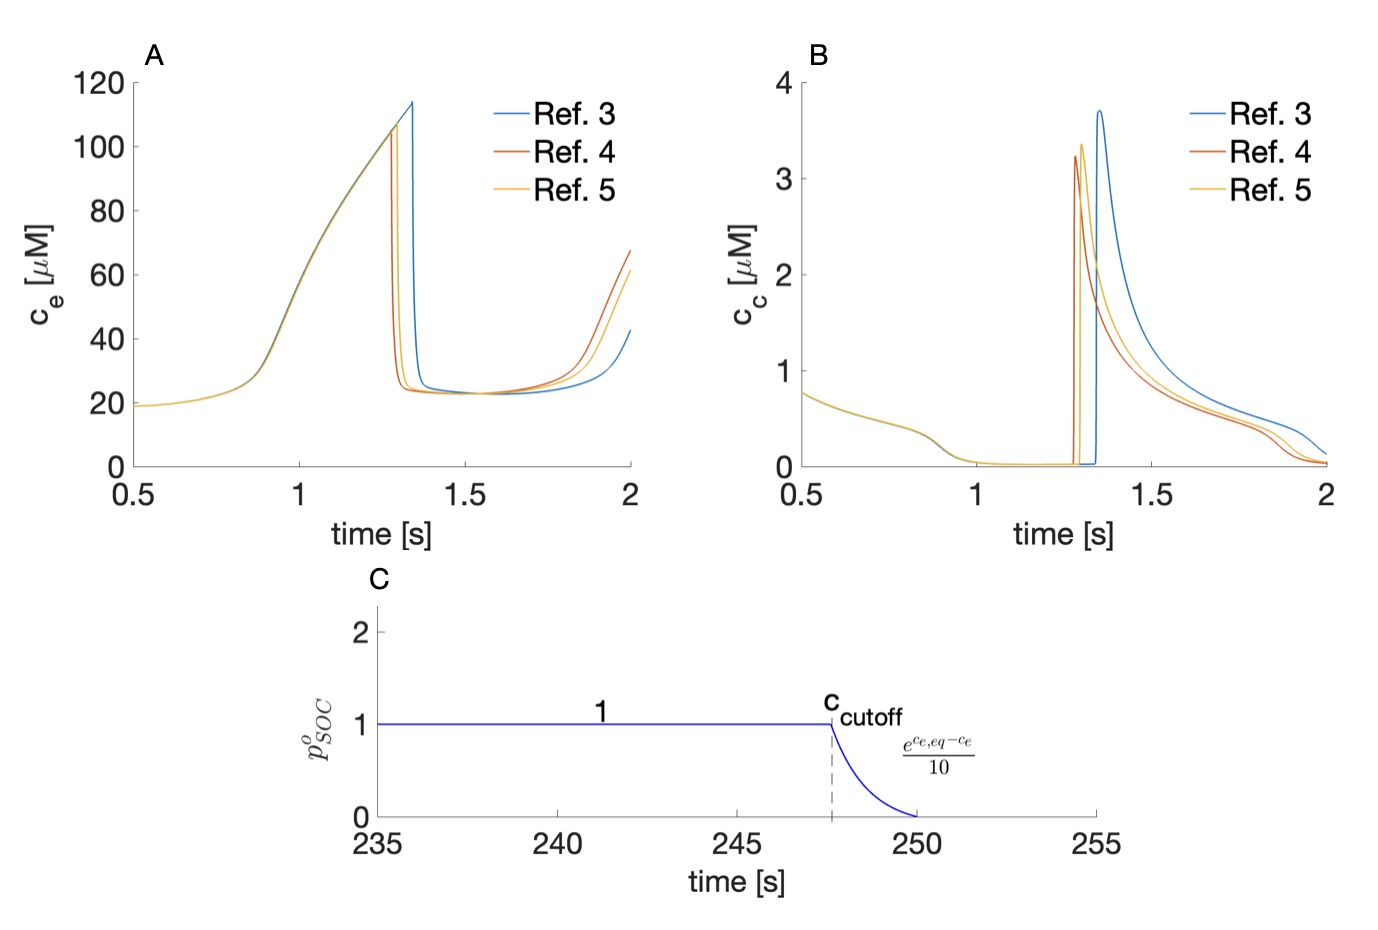
\includegraphics[width=12cm]{Figures/dxdt_posoc.png}
    \caption{Convergence analysis using different refinement levels. (A-B) concentration profiles for $Ca^{2+}$ in the cytosol and ER, respectively on an unbranched neurite. The refinement levels were $m=1,2,3,4,5$, with the edge length of $\Delta x = 2.0, 1.0, 0.5, 0.25, 0.125 ~\mu m$ and time step $\Delta t = 160, 80, 40, 20, 10~ms$, respectively. (C) open state probability of SOC ($p^o_{SOC}$) is modeled after eq.~\cref{eqn:posoc}. The value of $p^o_{SOC}$ is set to $1$ until it reaches a cutoff value ($247.602~\mu M$, calculated) after which it decays exponentially to zero.}
\end{figure}

\begin{figure}[!h]\label{fig:cc_andPory_supp}
    \centering
    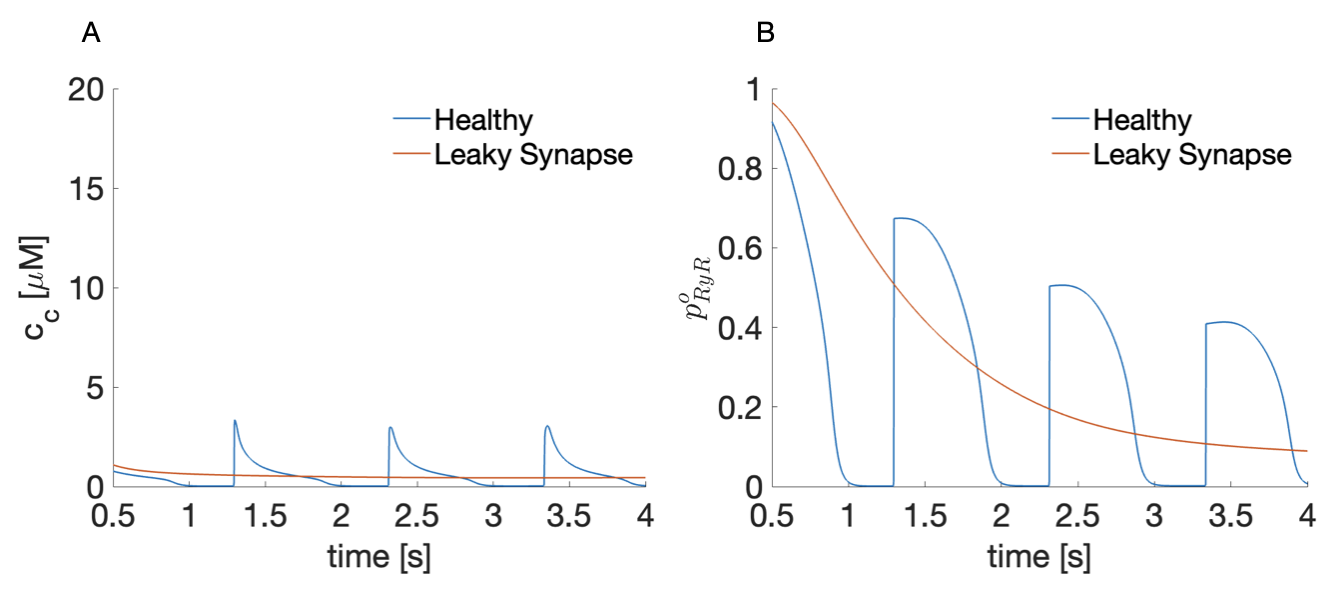
\includegraphics[width=12cm]{Figures/cc_andPory_supp.png}
    \caption{RyR open state probability in healthy vs. leaky synapse in an unbranched neurite with 5Hz stimulation. (A) The $Ca^{2+}$ profile at the soma in the healthy state causes 1Hz wave responses, where $c_c$ is low during equilibrium. In leaky synapses, baseline $c_c$ is elevated and no such wave response is observed. (B) The decrease of $c_c$ levels to baseline in the healthy state allows $p^o_{RyR}$ to also return to $0$ after a wave event. However, in case of leaky synapses, the elevated $c_c$ levels prevent $p^o_{RyR}$ to return to $0$ rapidly and thus hinders wave initiation.}
\end{figure}

\begin{figure}[!h]\label{fig:VDCCFig}
    \centering
    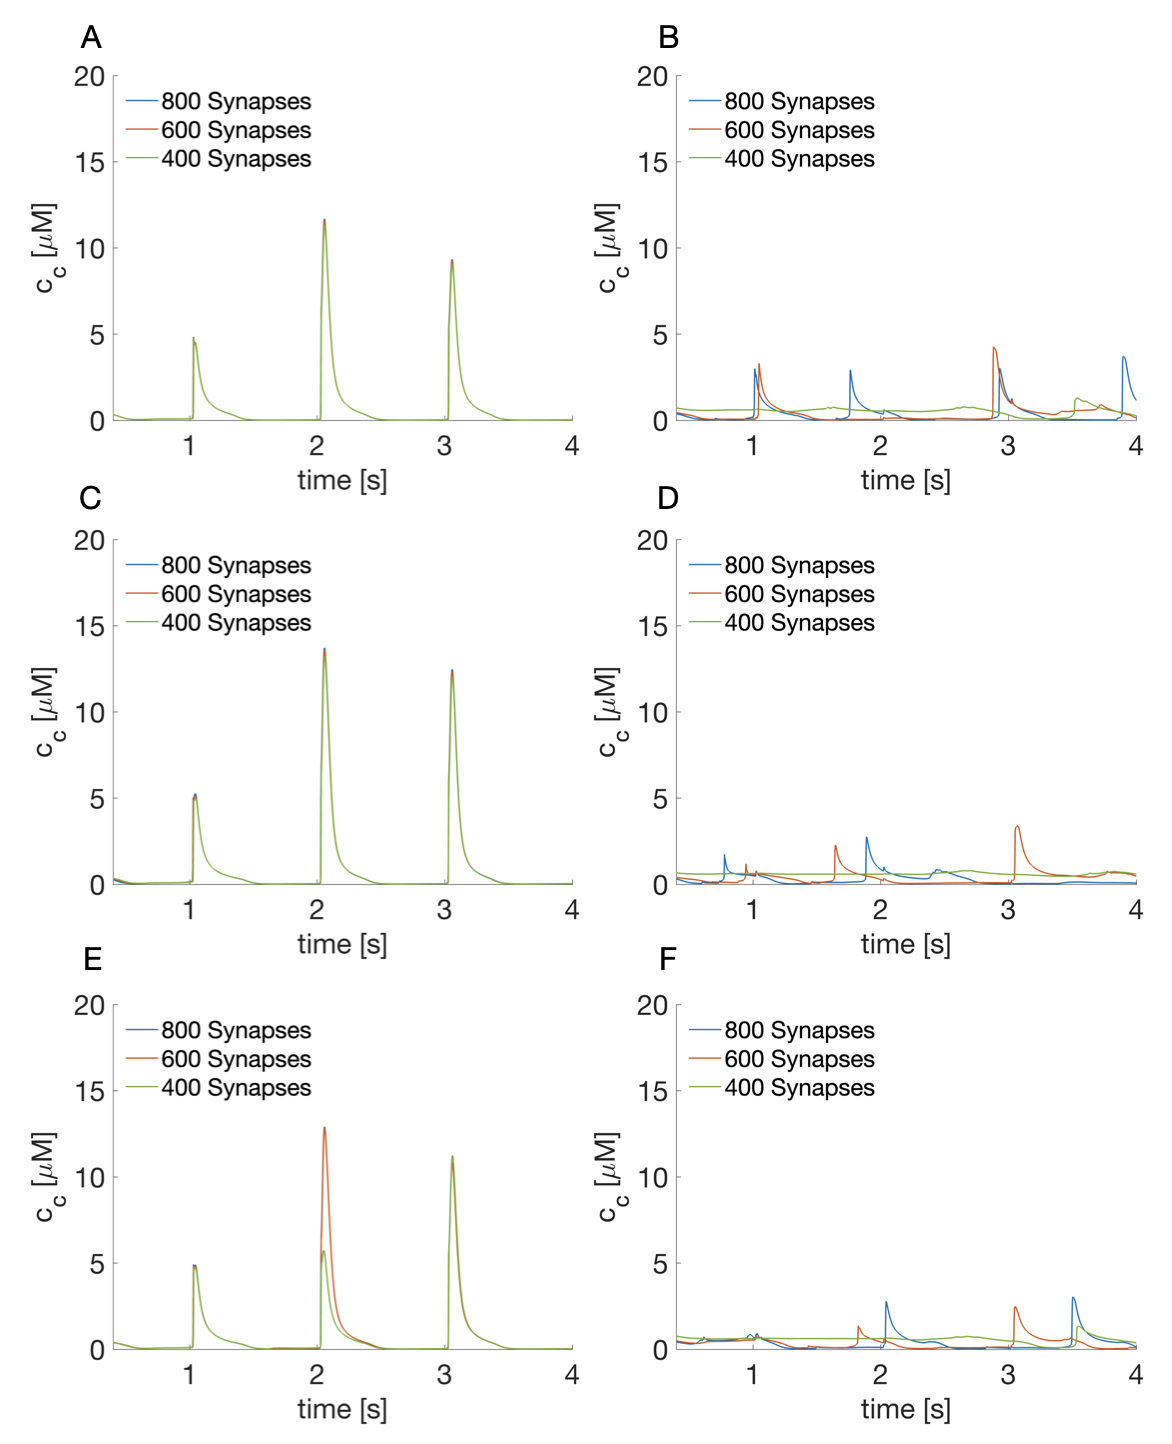
\includegraphics[width=12cm]{Figures/VDCCFig.png}
    \caption{Comparing different electro-calcium coupling. (A-B) no VDCCs, i.e., no eletrical coupling at 1Hz (A) and 5Hz (B) stimulation frequency. (C-D) N-Type VDCC coupling at 1Hz and 5Hz. (E-F) T-Type VDCC coupling at 1Hz and 5Hz. This figure is intended to illustrate that coupling the calcium dynamics to the electrical signal is relevant and different results are to be expected when excluding electro-calcium coupling or including different types of VDCC.} 
\end{figure}

\clearpage
\begin{table}[htbp]
{%\footnotesize
  \fontsize{6.5pt}{8.0pt}\selectfont
  \caption{Model Parameters}  \label{tab:modelparameters}
\begin{center}
  \begin{tabular}{|cccc|} \hline
   \bf Parameter & \bf Symbol & \bf Value & \bf Reference \\ \hline
    & \multicolumn{2}{c}{\textit{Initial and equilibrium values}}   &  \\
    Cytosolic \Ca &  \cc & $50~ nM$ & \cite{Queisser2018}\\
    ER \Ca & \ce & $250~ \mu M$ & \cite{Queisser2018}\\
    Reference ER \Ca & $c_e^{ref}$ & $250~ \mu M$ & \cite{Queisser2018}\\
    Extracellular \Ca & \co & $1~ mM$ & \cite{Queisser2018} \\
    Total Calbindin D$_{28k}$ (Cytosol) & \btot  & $40~ \mu M$ & \cite{muller2005endogenous,Queisser2018} \\
    Total Calreticulin (ER) & \betot &  $3.6~ mM$ & \cite{means2006reaction} \\
    &  & & \\
    & \multicolumn{2}{c}{\textit{Diffusion/reaction}}  &  \\
    Diffusion coefficient (\cc)  & \Dc & $220~ \mu m^2 s^{-1}$ & \cite{allbritton1992range,Queisser2018} \\
    Diffusion coefficient (CalB)  & \Dc & $20~ \mu m^2 s^{-1}$ & \cite{schmidt2003mutational,Queisser2018} \\
    CalB forward rate & $\kappa_b^+$ & $27~ \mu M^{-1}s^{-1}$ & \cite{muller2005endogenous,Queisser2018}\\
    CalB backward rate & $\kappa_b^-$ & $19~ s^{-1}$ & \cite{muller2005endogenous,Queisser2018}\\
    Diffusion coefficient (\ce)  & \Dce & $10~ \mu m^2 s^{-1}$ & \cite{dayel1999diffusion,mcivor2018three} \\
    Diffusion coefficient (CalR)  & \Dbe & $27~ \mu m^2 s^{-1}$ & \cite{means2006reaction} \\
    CalR forward rate & $\kappa_{be}^+$ & $10^5~ M^{-1}s^{-1}$ & \cite{means2006reaction}\\
    CalR backward rate & $\kappa_{be}^-$ & $200~ s^{-1}$ & Calculated using \\ 
    &  & & $K_d = 2~mM$ (\cite{baksh1991expression})\\
    &  & & \\
    & \multicolumn{2}{c}{\textit{RyR channel}}   & \\
    $o_1 \to c_1$ &  $k_a^-$ & $28.8~ s^{-1}$ & \cite{Keizer1996}\\
    $c_1 \to o_1$ &  $k_a^+$ & $1500~ \mu M^{-4}s^{-1}$ & \cite{Keizer1996}\\
    $o_2 \to o_1$&  $k_b^-$ & $385.9~ s^{-1}$ & \cite{Keizer1996}\\
    $o_1 \to o_2$&  $k_b^+$ & $1500~ \mu M^{-3}s^{-1}$ & \cite{Keizer1996}\\
    $c_2 \to o_1$&  $k_c^-$ & $0.1~ s^{-1}$ & \cite{Keizer1996}\\
    $o_1 \to c_2$&  $k_c^+$ & $1.75~ s^{-1}$ & \cite{Keizer1996}\\
    Reference current & $I_{RyR}^{ref}$ & $3.5 \times 10^{-18}~ mol~s^{-1}$& \cite{Tinker1993}\\ 
    &  & & \\
    & \multicolumn{2}{c}{\textit{SERCA pumps}}   & \\
    SERCA current &  $I_S$ & $6.5 \times 10^{-21}~ mol~\mu M~s^{-1}$ & \cite{chiu1980rapid,Queisser2018}(Adapt.)\\
    & $K_S$  & $180~ nM$ & \cite{Sneyd2003}\\
    SERCA density & $\rho_S$ & $2390~ \mu m^{-2}$ & \cite{means2006reaction}(Approx.)\\
    &  & & \\
    & \multicolumn{2}{c}{\textit{PMCA pumps}} & \\
    PMCA current &  $I_P$ & $1.7 \times 10^{-23}~ mol~s^{-1}$ & \cite{Graupner2003}\\
    Measure of \Ca affinity & $K_P$  & $ 60~ nM$ & \cite{elwess1997plasma}\\
    PMCA density & $\rho_P$ & $500~ \mu m^{-2}$ & \cite{Queisser2018}(Estim.)\\
    &  & & \\
    & \multicolumn{2}{c}{\textit{NCX pumps}} & \\
    NCX current &  $I_N$ & $2.5 \times 10^{-21}~ mol~s^{-1}$ & \cite{Graupner2003}(adapt.)\\
    Measure of \Ca affinity & $K_N$  & $ 1.8~ \mu M$ & \cite{Graupner2003}\\
    NCX density & $\rho_N$ & $15~ \mu m^{-2}$ & \cite{Queisser2018}(Estim.)\\
    &  & & \\
    &  \multicolumn{2}{c}{\textit{Store Operated Channels}} & \\
    Single SOC current &  $I^{ref}_{SOC}$ & $2.1~ fA$ & \cite{gil2021three,hoth1992depletion}\\
    Faraday's Constant & $F$ & $96485~ C/mol$ & \\
    Valency of \Ca ~ion & $z$ & 2 & \\
    Density of SOC & $\rho_{SOC}$ & $0.4 ~\mu m^{-2}$ & choosen\\
    &  & & \\
    &\multicolumn{2}{c}{\textit{A$\beta$ pores}} & \\
    Rate constant & $k_{\beta}$ & $1~ s^{-1}$ & \cite{latulippe2018mathematical,de2013progression}\\
    Cooperative factor & $m$ & $4$ & \cite{latulippe2018mathematical,de2013progression}\\
    Concentration of A$\beta$ & a & $5 ~nM$, $100 ~\mu M$ & \cite{de2013progression,paula2011amyloid}\\
    & & &\\
    %&  \textit{Leakages} & & \\
    %Leakage velocity ERM & $v_{l,e}$ & $~ nm~s^{-1} $ & (Calc.)\\
    %Leakage velocity PM & $v_{l,p}$ & $~ nm~s^{-1} $ & (Calc.) \\
    %& & &\\
    & \multicolumn{2}{c}{\textit{Miscellaneous}} & \\
    Input synaptic flux & $j_{syn}$ & $1 \times 10^{-6}~ $ & \cite{Queisser2018,rosado2022}\\
    &  & & \\ \hline
  \end{tabular}
\end{center}
}
\end{table}

\clearpage
\begin{table}[ht] 
{
   \fontsize{6.5pt}{8.0pt}\selectfont
   \caption{Model Parameters for VDCCs and electrical dynamics equations}
    \begin{center}
    \begin{tabular}{|cccc|}\hline
    \bf Parameter & \bf Symbol & \bf Value & \bf Reference \\ \hline
          &  \multicolumn{2}{c}{\textit{Voltage Dependent Calcium Channels (VDCC) N-type}} & \\
          Valence &$z_k, z_l$  & 2, 1 & \cite{Grein2014,BorgGraham1999} \\
          Voltage &$V_{1/2,k},V_{1/2,l}$  &  -21 $mV$, -40 $mV$ & \cite{Grein2014,BorgGraham1999} \\
          Rate parameter& $\gamma_k, \gamma_l$ & 0, 0 & \cite{Grein2014,BorgGraham1999} \\
          Rate parameter& $K_k, K_l$ & 1.7 $ms$, 70 $ms$ & \cite{Grein2014,BorgGraham1999}\\
          Time constant & $\tau_{0,k}, \tau_{0,l}$ & 1.7 $ms$, 70 $ms$ & \cite{Grein2014,BorgGraham1999}\\
          Permeability of \Ca & $\bar{p}_{\textrm{Ca}^{2+}}$ & 3.8 $cm^3$/s& \cite{Grein2014,BorgGraham1999}\\
          Faraday Constant & $F$ & 96485 C/mol & \cite{Grein2014,BorgGraham1999}\\
          Gas Constant & $R$ & 8.314 $J/K$mol & \cite{Grein2014,BorgGraham1999}\\
          Temperature & $T$ & 310 Kelvin & \cite{Grein2014,BorgGraham1999}\\
          & & &\\
          &  \multicolumn{2}{c}{\textit{Voltage Dependent Calcium Channels (VDCC) T-type}} & \\
          Valence &$z_k, z_l$  & 2,1 &  \cite{BorgGraham1999} \\
          Voltage &$V_{1/2,k},V_{1/2,l}$  &  -36 $mV$, -68 $mV$ &  \cite{BorgGraham1999} \\
          Rate parameter& $\gamma_k, \gamma_l$ & 0,0 & \cite{BorgGraham1999} \\
          Rate parameter& $K_k, K_l$ & 1.5 $ms$ ,10 $ms$  & \cite{BorgGraham1999}\\
          Time constant & $\tau_{0,k}, \tau_{0,l}$ & 1.5 $ms$, 10 $ms$ & \cite{BorgGraham1999}\\
          Permeability of \Ca & $\bar{p}_{\textrm{Ca}^{2+}}$ & 1.9 $cm^3$/s & \cite{Grein2014,BorgGraham1999}\\
          & & &\\
          % &  \multicolumn{2}{c}{\textit{Voltage Dependent Calcium Channels (VDCC) L-type}} & \\
          % Valence &$z_k, z_l$  &  & \cite{BorgGraham1999} \\
          % Voltage &$V_{1/2,k},V_{1/2,l}$  &   & \cite{BorgGraham1999} \\
          % Rate parameter& $\gamma_k, \gamma_l$ & & \cite{BorgGraham1999} \\
          % Rate parameter& $K_k, K_l$ &  & \cite{BorgGraham1999}\\
          % Time constant & $\tau_{0,k}, \tau_{0,l}$ & & \cite{BorgGraham1999}\\
          % Permeability of \Ca & $\bar{p}_{\textrm{Ca}^{2+}}$ & & \cite{Grein2014,BorgGraham1999}\\
          % & & &\\
          &\multicolumn{2}{c}{\textit{Parameters for Electrical Dynamics}}&\\
          Axonal Resistance & $R_{ax}$  & 0.75 $\Omega\cdot m$&\cite{Pospischil2008} \\
          Membrane Capacitance & $C$ & 0.01 $F/m^2$& \cite{Pospischil2008}\\
          K$^{+}$ Conductance &$\Bar{g}_{K}$ & 50 $S/m^2$& \cite{Pospischil2008}\\
          Na$^{2+}$ Conductance & $\Bar{g}_{Na}$ & 500 $S/m^2$ & \cite{Pospischil2008}\\
          Leak Conductance &$\Bar{g}_{l}$ & 0.05 $S/m^2$ & \cite{Pospischil2008}\\
          K$^{+}$ Reversal Potential & $V_{K}$& -0.90 $V$ &  \cite{Pospischil2008}\\
          Na$^{2+}$ Reversal Potential & $V_{Na}$& 0.50 $V$ & \cite{Pospischil2008}\\
          Leak Reversal Potential & $V_l$& -0.60 $V$ &  \cite{Pospischil2008}\\
          \Ca Reversal Potential & $V_{Ca}$ & A function of \Ca & \cite{proto1998,koch1989methods} \\
          Initial K$^{+}$ Channel Probability & $n_0$ & 0.00654 & \cite{Hodgkin1952A}\\
          Initial Na$^{2+}$ Channel Probability & $m_0$  & 0.00654 &\cite{Hodgkin1952A}\\
          Initial Na$^{2+}$ Channel Probability & $h_0$  & 0.9997 & \cite{Hodgkin1952A}\\
          Initial \Ca Channel Probability &$\sigma_0$ & 0.9750 & \cite{proto1998,koch1989methods}\\
          Calcium Current Parameter & $K$ & 0.01 mol$/m^3$& \cite{proto1998,koch1989methods} \\
          & & &\\
          \hline          
    \end{tabular}
    \end{center}
}
\end{table}\label{tab:otherparameters}

\newpage
\section{Derivation for $1$D reduced model}
In this section, we derive the $1$D reduced PDEs for cytosolic \Ca concentration $c_c$. Fig. \ref{fig:Illustration_Supp} illustrates a section of unbranched neurite of width $dx$. The ER radius and the dendrite radius are denoted by $r$ and $R$ respectively. The fluxes ($J_{PM}$) between cytosolic ($\Omega_{C}$) and extracellular domain are on boundary $\Gamma_{PM}$ while the fluxes ($J_{ERM}$) between ER ($\Omega_{ER}$) and cytosolic doamins are on boundary $\Gamma_{ERM}$. At a given point, surface area of $\Gamma_{PM}=2\pi R$ and $\Gamma_{ERM}=2\pi r$. The area of $\Omega_{C}=\pi(R^2-r^2)$ and $\Omega_{ER}=\pi r^2$.

\begin{figure}[H]\label{fig:Illustration_Supp}
    \centering
    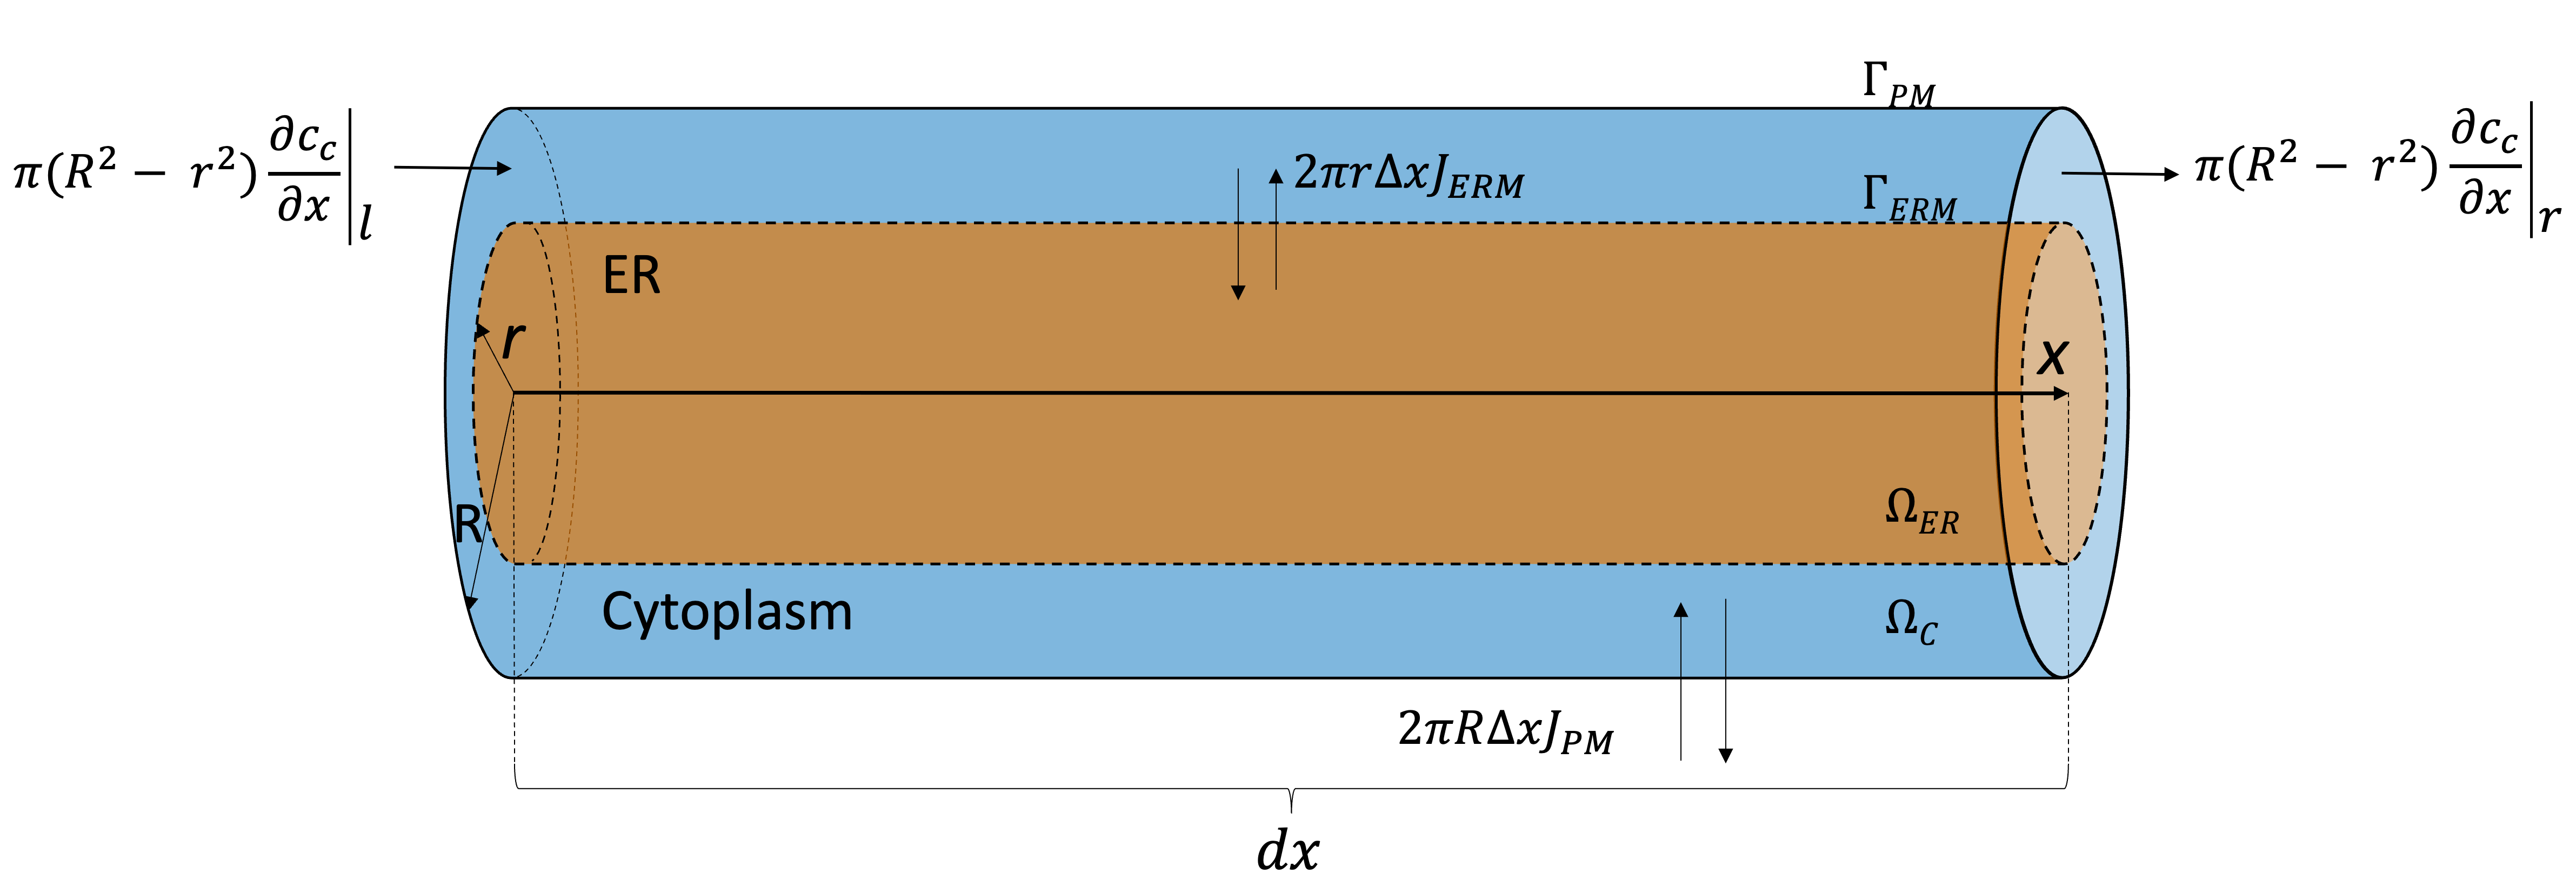
\includegraphics[width=\textwidth]{Figures/Illustration_Supp.png}
    \caption{Illustration of a section of an unbranched neurite of width $dx$ displaying mechanisms affecting cytosolic \Ca concentration.} 
\end{figure}

We begin with the flux balance equation where each flux is scaled by the corresponding area/volume:
\begin{eqnarray*}
    \pi(R^2-r^2)\Delta x \frac{\partial c_c}{\partial t} &=& \left(\pi (R^2-r^2) \frac{\partial c_c}{\partial x} \middle\vert_r - \pi (R^2-r^2) \frac{\partial c_c}{\partial x} \middle\vert_l \right) + 2\pi r\Delta x J_{ERM} \\
    &&  + 2\pi R \Delta x J_{PM} + \pi (R^2-r^2)(k_b^-(b^{tot}-b)-k_b^+bc_c)\\
    (R^2 - r^2) \frac{\partial c_c}{\partial t} &=& \frac{\left( (R^2-r^2) 
 \frac{\partial c_c}{\partial x}\middle\vert_r - (R^2-r^2) 
 \frac{\partial c_c}{\partial x}\middle\vert_l \right)}{\Delta x} \\ 
  && + (R^2-r^2)(k_b^-(b^{tot}-b)-k_b^+bc_c)+ 2rJ_{ERM} + 2RJ_{PM}
\end{eqnarray*}

Dividing by $\Delta x$ and taking $\Delta x$ to $0$ leads to:
\begin{eqnarray*}
    (R^2 - r^2) \frac{\partial c_c}{\partial t} &=& \frac{\partial}{\partial x}\left((R^2-r^2) \frac{\partial c_c}{\partial x}\right) + (R^2-r^2)(k_b^-(b^{tot}-b)-k_b^+bc_c) \\
    && + 2rJ_{ERM} + 2RJ_{PM}\\
    \frac{\partial c_c}{\partial t} &=& \frac{1}{(R^2 - r^2)} \frac{\partial}{\partial x}\left((R^2 - r^2) \frac{\partial c_c}{\partial x}\right) + (k_b^-(b^{tot}-b)-k_b^+bc_c) \\
    && +\frac{2r}{R^2-r^2}J_{ERM} + \frac{2R}{R^2-r^2}J_{PM}, \qquad \text{in $\Omega_{C}$}
\end{eqnarray*}

Equivalently, we derive the 1D reduced equations for $c_e$, $b$ and $b_e$:

\begin{eqnarray*}
    \frac{\partial c_e}{\partial t}&=&\frac{1}{r^2}\frac{\partial}{\partial x}\left(r^2D_c\frac{\partial c_e}{\partial x}\right) + \left(k_{be}^-(b_e^{tot}-b_e)-k_{be}^+b_ec_e\right) \\ \notag \\
    && -\frac{2}{r}J_{ERM} + \frac{2}{r}J_{SOC}, \qquad \text{in $\Omega_{ER}$} \notag \\ \notag \\
    \frac{\partial b}{\partial t}&=&\frac{1}{(R^2-r^2)}\frac{\partial}{\partial x}\left((R^2-r^2)D_b\frac{\partial b}{\partial x}\right)+\left(k_b^-(b^{tot}-b)-k_b^+bc_c\right), \qquad \text{in $\Omega_{C}$}\\  \notag \\
    \frac{\partial b_e}{\partial t}&=&\frac{1}{r^2}\frac{\partial}{\partial x}\left(r^2D_{be}\frac{\partial b_e}{\partial x}\right)+\left(k_{be}^-(b_e^{tot}-b_e)-k_{be}^+b_ec_e\right) \qquad \text{in $\Omega_{ER}$}%\\  \notag \\
\end{eqnarray*}

\bibliographystyle{siamplain}
\bibliography{references}
\end{document}
